\documentclass[12pt,a4paper,onecolumn]{article}
\usepackage[utf8]{inputenc}
\usepackage[T1]{fontenc}
\usepackage[french]{babel}

% ------------------------- Color table ----------------------------------------
\usepackage{multirow}
\usepackage[table]{xcolor}
\definecolor{maroon}{cmyk}{0,0.87,0.68,0.32}
% ------------------------------------------------------------------------------

\usepackage{amscd}
\usepackage{amsthm}
\usepackage{physics}
\usepackage[left=2.2cm,right=2.2cm,top=2cm,bottom=2cm]{geometry}
\usepackage{textcomp,gensymb} %pour le °C, et textcomp pour éviter les warning
\usepackage{graphicx} %pour les images
\usepackage{caption}
\usepackage{subcaption}
\usepackage[colorlinks=true,
	breaklinks=true,
	citecolor=blue,
	linkcolor=blue,
	urlcolor=blue]{hyperref} % pour insérer des liens
\usepackage{epstopdf} %converting to PDF
\usepackage[export]{adjustbox} %for large figures

\usepackage{array}
\usepackage{dsfont}% indicatrice : \mathds{1}


% -------------------------- Mathematics ---------------------------------------
\graphicspath{{images/}} % For the images path
% ------------------------------------------------------------------------------

% -------------------------- Mathematics ---------------------------------------
\usepackage{mathrsfs, amsmath, amsfonts, amssymb}
\usepackage{bm}
\usepackage[Symbol]{upgreek} % For pi \uppi different from /pi
\newcommand{\R}{\mathbb{R}} % For Real space
% ------------------------------------------------------------------------------


% -------------------------- Code format ---------------------------------------
\usepackage[numbered,framed]{matlab-prettifier}
\lstset{
	style              = Matlab-editor,
	basicstyle         = \mlttfamily,
	escapechar         = '',
	mlshowsectionrules = true,
}
% ------------------------------------------------------------------------------

% ------------------------- Blbiographie --------------------------------------
% \usepackage[backend=biber, style=science]{biblatex}
% \addbibresource{biblio.bib}
% ------------------------------------------------------------------------------


\setcounter{tocdepth}{4} %Count paragraph
\setcounter{secnumdepth}{4} %Count paragraph
\usepackage{float}

\usepackage{graphicx} % for graphicspath
% \graphicspath{{../images/}}

\usepackage{array,tabularx}
\newcolumntype{L}[1]{>{\raggedright\let\newline\\\arraybackslash\hspace{0pt}}m{#1}}
\newcolumntype{C}[1]{>{\centering\let\newline\\\arraybackslash\hspace{0pt}}m{#1}}
\newcolumntype{R}[1]{>{\raggedleft\let\newline\\\arraybackslash\hspace{0pt}}m{#1}}

\title{Matrice Fondamentale}
\author{Vincent Matthys}


\renewcommand{\thesubsection}{\alph{subsection}}


\begin{document}
%\maketitle
\begin{tabularx}{\textwidth}{@{} l X r @{} }
	{\textsc{Master MVA}}          &  & \textsc{Scnenario d'usage} \\
	\textsc{UE 3D COMPUTER VISION} &  & {ENS Paris Saclay}         \\
	%& %M1 Informatique
\end{tabularx}
\vspace{1.5cm}
\begin{center}

	\rule[11pt]{5cm}{0.5pt}

	\textbf{\LARGE \textsc{Détermination de la matrice Fondamentale par algorithme ransac}}
	\vspace{0.5cm}

	Vincent Matthys


	\rule{5cm}{0.5pt}

	\vspace{1.5cm}
\end{center}

\section{Objectif}
Le programme permet à l'utilisateur :
\begin{enumerate}
	\item de déterminer la matrice fondamentale à partir de deux images d'une même scène sans connaissance au préalable des paramètres internes de l'appareil.
	\item de tracer la ligne épipolaire associé à un point sélectionné par l'utilisateur dans l'autre image.
\end{enumerate}


\section{Material \& Method}
Un seul fichier C++, nommé \textit{Fundamental.cpp} charge et affiche les deux images, qui peuvent être passés en paramètres du programme nommé \textit{Fundamental}. Un algorithme déterminant les SIFT est alors lancé sur chaque image, et les correspondances entre SIFT sont enregistrées.

Ces correspondances sont alors épurées par RANSAC, en calculant une matrice fondamentale avec l'algorithme des 8 points, et en discriminant les correspondances déterminées par SIFT matching en calculant la distance d'un point d'une correspondance à sa droite épipolaire associée. Si celle-ci est inférieure à \(10^{-5}\), alors la correspondance est considérée comme \textit{inlier}. Ce critère de distance a été retenu afin d'obtenir avec une certitude de \( \beta = 1~\%\) d'obtenir 8 correspondances non contaminées par des correspondances aberrantes par tirage aléatoire, en une trentaine d'itérations, ne gardant que \( 500\) correspondances sur les \( 675 \) retournées par SIFT matching.

L'algorithme des 8 points consiste à résoudre le système linéaire suivant :

\begin{equation*}
	\begin{split}
		A \dotproduct f = 0\\
		\begin{bmatrix}
			A_1^{\intercal} \\
			A_2^{\intercal} \\
			A_3^{\intercal} \\
			A_4^{\intercal} \\
			A_5^{\intercal} \\
			A_6^{\intercal} \\
			A_7^{\intercal} \\
			A_8^{\intercal} \\
		\end{bmatrix}
		\dotproduct
		\begin{bmatrix}
			f_{11} \\
			f_{12} \\
			f_{13} \\
			f_{21} \\
			f_{22} \\
			f_{23} \\
			f_{31} \\
			f_{32} \\
			f_{33}
		\end{bmatrix}
		&=
		0\\
		\begin{bmatrix}
			x_1x_1^{\prime} & x_1y_1^{\prime} & x_1 & y_1x_1^{\prime} & y_1y_1^{\prime} & y_1 & x_1^{\prime} & y_1^{\prime} & 1 \\
			x_2x_2^{\prime} & x_2y_2^{\prime} & x_2 & y_2x_2^{\prime} & y_2y_2^{\prime} & y_2 & x_2^{\prime} & y_2^{\prime} & 1 \\
			x_3x_3^{\prime} & x_3y_3^{\prime} & x_3 & y_3x_3^{\prime} & y_3y_3^{\prime} & y_3 & x_3^{\prime} & y_3^{\prime} & 1 \\
			x_4x_4^{\prime} & x_4y_4^{\prime} & x_4 & y_4x_4^{\prime} & y_4y_4^{\prime} & y_4 & x_4^{\prime} & y_4^{\prime} & 1 \\
			x_5x_5^{\prime} & x_5y_5^{\prime} & x_5 & y_5x_5^{\prime} & y_5y_5^{\prime} & y_5 & x_5^{\prime} & y_5^{\prime} & 1 \\
			x_6x_6^{\prime} & x_6y_6^{\prime} & x_6 & y_6x_6^{\prime} & y_6y_6^{\prime} & y_6 & x_6^{\prime} & y_6^{\prime} & 1 \\
			x_7x_7^{\prime} & x_7y_7^{\prime} & x_7 & y_7x_7^{\prime} & y_7y_7^{\prime} & y_7 & x_7^{\prime} & y_7^{\prime} & 1 \\
			x_8x_8^{\prime} & x_8y_8^{\prime} & x_8 & y_8x_8^{\prime} & y_8y_8^{\prime} & y_8 & x_8^{\prime} & y_8^{\prime} & 1
		\end{bmatrix}
		\dotproduct
		\begin{bmatrix}
			f_{11} \\
			f_{12} \\
			f_{13} \\
			f_{21} \\
			f_{22} \\
			f_{23} \\
			f_{31} \\
			f_{32} \\
			f_{33}
		\end{bmatrix}
		&=
		\begin{bmatrix}
			\vdots \\
			0      \\
			\vdots
		\end{bmatrix}
	\end{split}
\end{equation*}

Avec la contrainte \( \norm{f} = 1\). \( f\) est alors le dernier vecteur singulier à droite de la matrice \( A\). Le programme utilise une décomposition \(SVD\) carré en rajoutant l'équation \( 0 = 0\) comme dernière ligne de \(A\), ce qui implique alors le choix de l'avant dernier vecteur singulier à droite.

La matrice fondamentale est finalement calculée sur les \textit{inliers} restant déterminés par \textit{RANSAC} par minimization de l'erreur quadratique. du système précédemment présenté, avec \( f_{33} = 1\). Après décomposition \(SVD\), la dernière valeur singulière est mise à 0 pour forcer le rang de \( f\) à 2. \(f\) est ensuite recomposée.

Il faut noter que le calcul de \(f\) nécessite une normalization des échelles, qui est inversée après calcul. Cette normalization consiste à multiplier toutes de coordonnées par \( 10^{-3} \) pour ramener l'échelle autour de l'unité, pour des images de l'ordre du millier de pixels de dimension.

\end{document}


%
% To successfully finds H, the system requires at least 4 correspondences, each one giving two equations. If there is more than 4 correspondences, the program solves the system using least squares programming.
% A sanity check is introduced and allows user the homography found. Every line should be $(0, 0, 0)$ vector. In reality, it is only close to the null vector, because, in particular, of errors during selection of points and the intrinsic noise of the camera.
%
% To build the panorama, the program uses the pull method, which requires to inverse the homography, and queries the preimage by H, which is the image by H, of each pixel in the final image. If it lies in the first image, then the pixel is pulled in the final image. In the overlapping area, the program simply averages the value of the two images.
%
% \section{Results}
% We present here 3 use cases obtained with the default images :
% \begin{enumerate}
% 	\item first view, left of the scene. Size : 755 x 499
% 	\item second view, right of the scene. Size : 755 x 499
% \end{enumerate}
%
% \subsection{Wrong use case}
%
% \subsubsection{Not enough correspondences}
%
% When the user doesn't give enough correspondences, the sanity check doesn't display, since the linear system can't be solved. Moreover, the homography is given, by default, as the identity matrix. Hence the panorama constructed in figure \ref{not_enough} is only the average of both image, as if they were taken with the same view.
% \begin{figure}[H]
% 	\begin{center}
% 		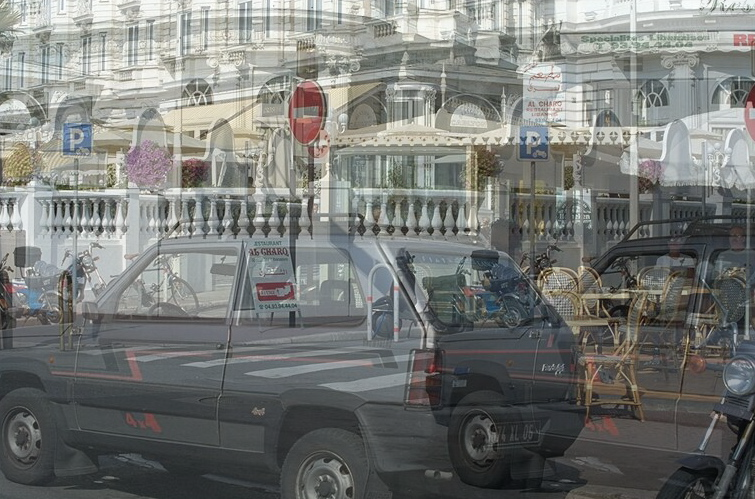
\includegraphics[width = \textwidth]{panorama_not_enough.png}
% 	\end{center}
% 	\caption{Panorama construction with not enough correspondences. Size : 755 x 499}
% 	\label{not_enough}
% \end{figure}
%
% \subsubsection{Wrong correspondences}
%
% When the user doesn't take proper correspondances, the homography found relies on wrong correspondances, hence a obvious wrong panorama construction, with geometric deformations.
% In the case presented in figure \ref{wrong_corr}, we can see those deformations and the homography found is the following :
%
% $$ H =
% 	\begin{bmatrix}
% 		0.792  & -0.281 & -279 \\
% 		-0.040 & 0.250  & 100  \\
% 		0.00   & 0.00   & 1
% 	\end{bmatrix}
% $$
%
% \begin{figure}[H]
% 	\begin{center}
% 		\frame{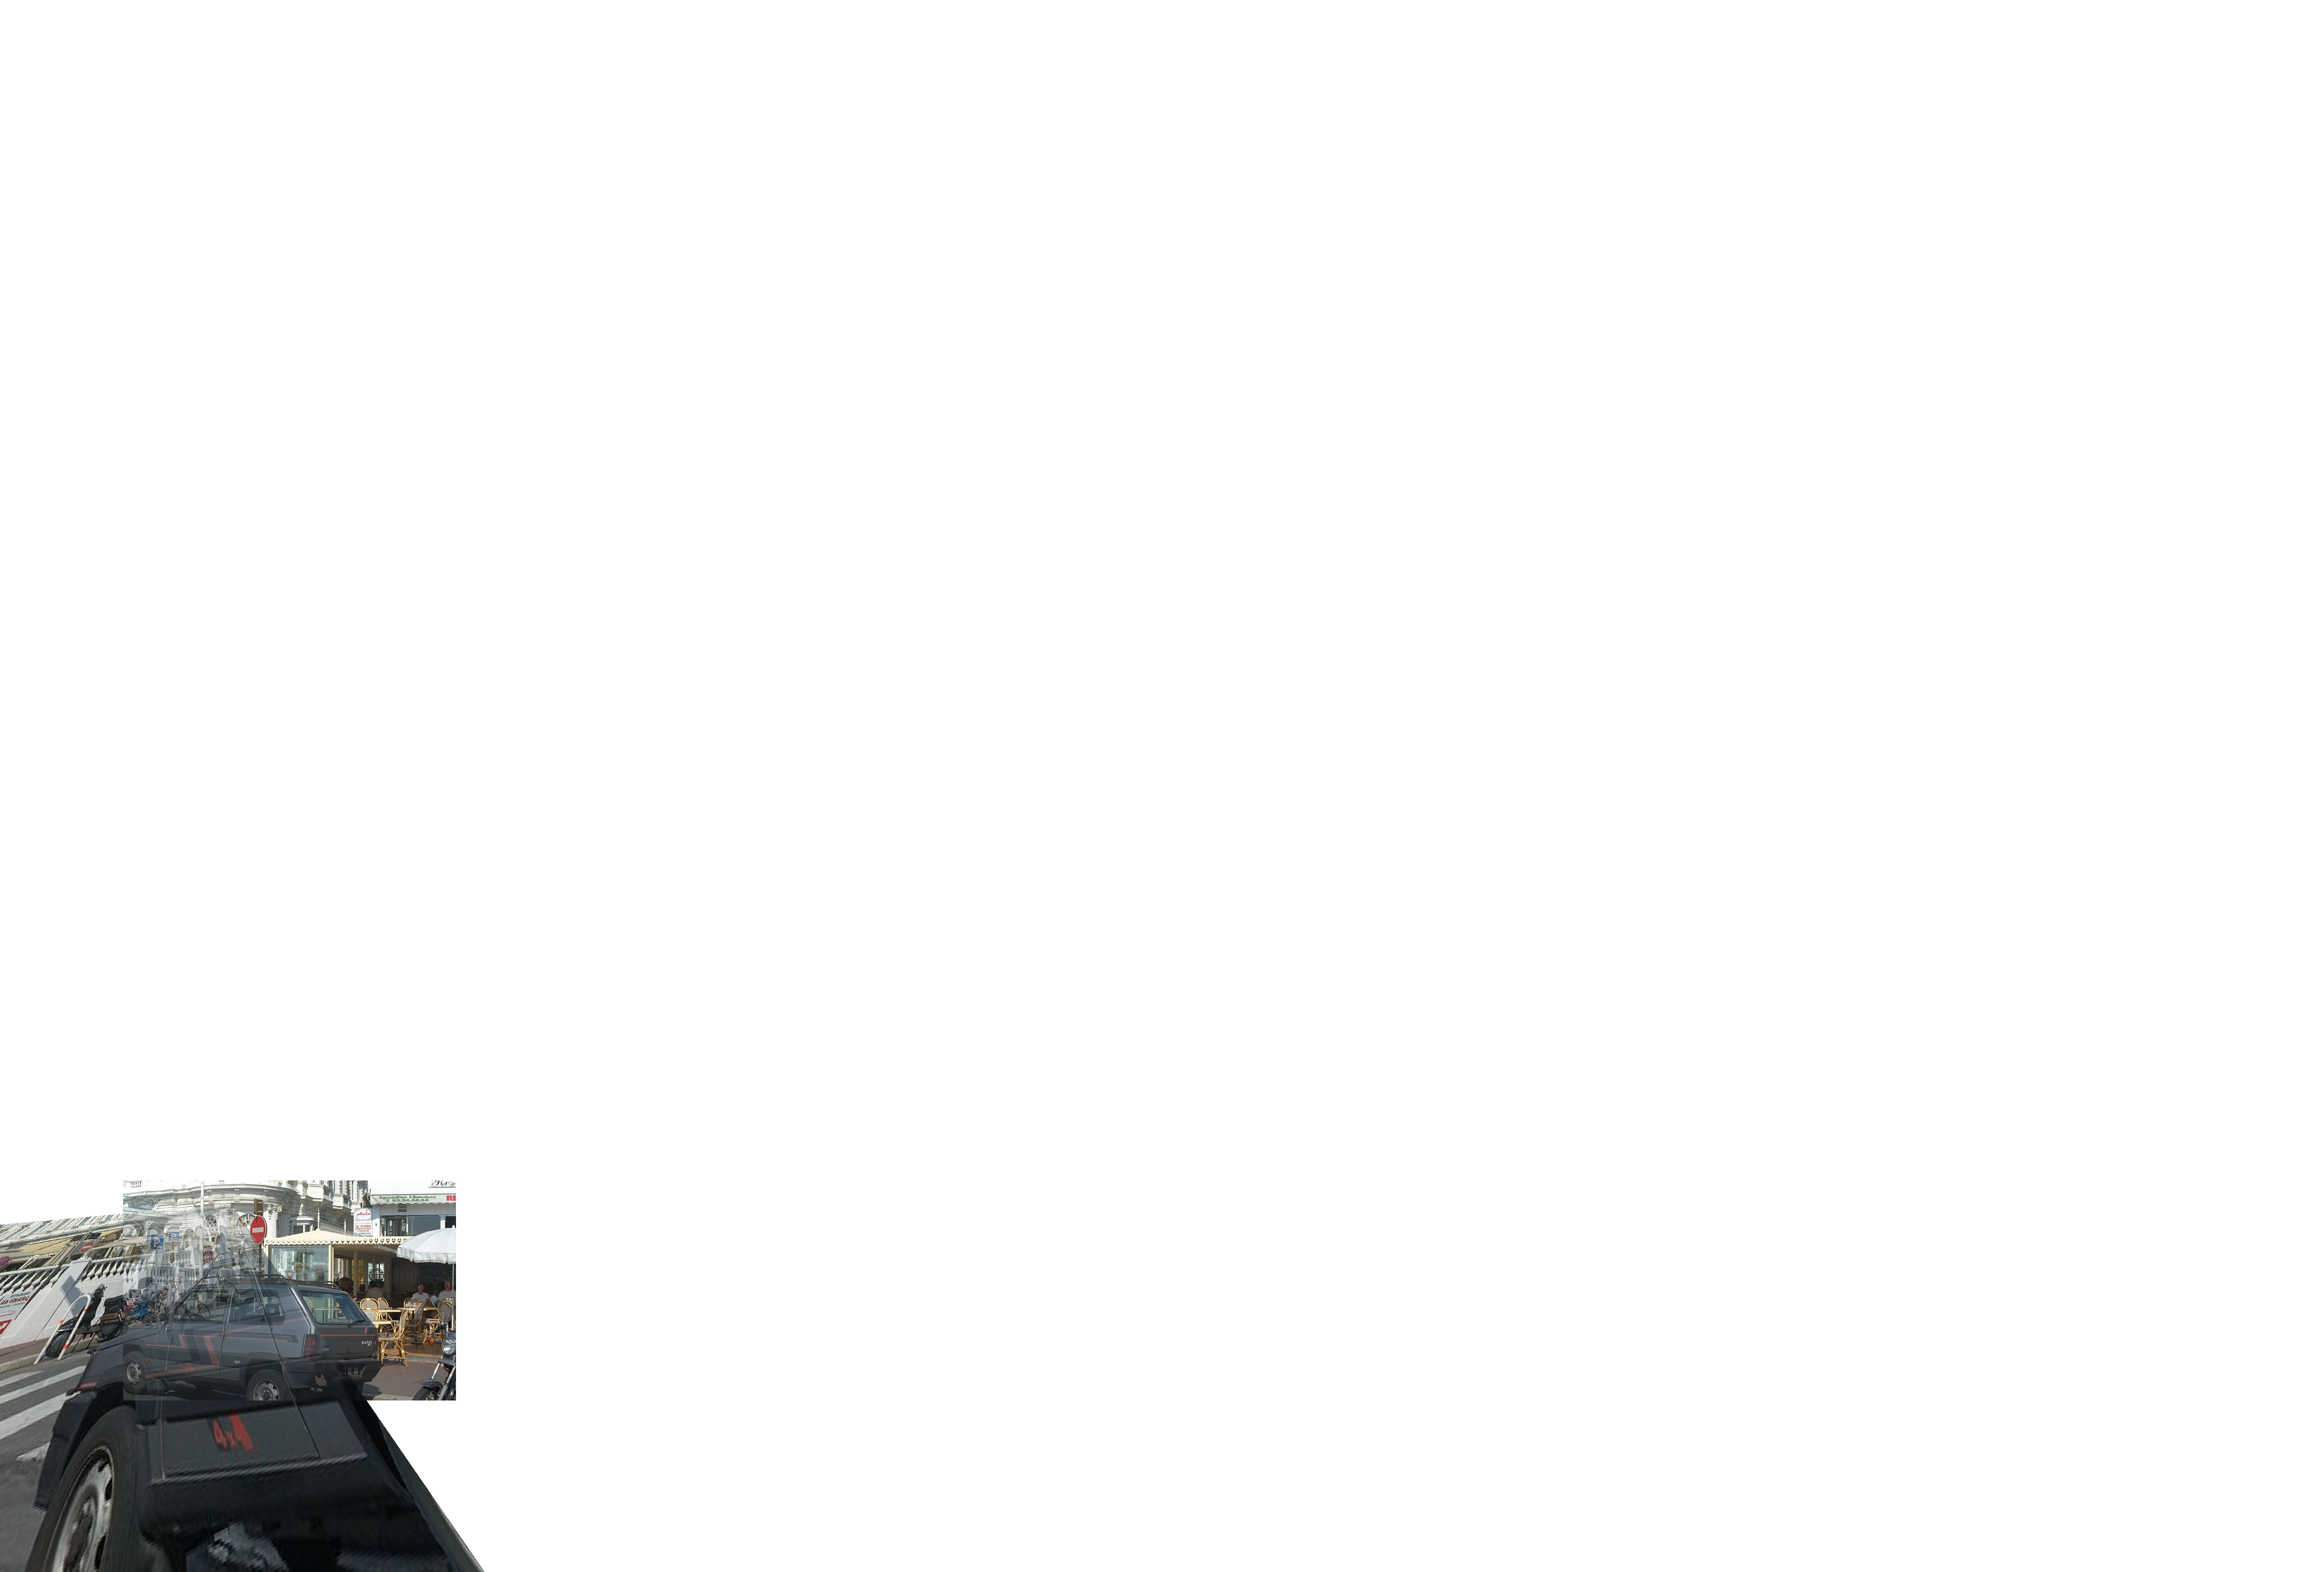
\includegraphics[width = \textwidth]{panorama_wrong_corr.png}}
% 	\end{center}
% 	\caption{Panorama construction with obvious wrong correspondences. A frame has been added to see the image size of the panorama : 5270 x 3565}
% 	\label{wrong_corr}
% \end{figure}
%
% \subsection{With 4 correspondences}
%
% In figure \ref{mini_corr}, a minimum number of 4 correspondences allows to find a proper homography between the two views. The overlapping area still remains a little blurred, and the panorama construction highlights is not rectangular, which shows that the homography found, given below is not perfect. Moreover, we can notice some aliasing on vertical lines on the pulled image.
%
% $$ H =
% 	\begin{bmatrix}
% 		1.02   & 7.36e-5 & -468 \\
% 		0.0120 & 1.02    & -8   \\
% 		0.00   & 0.00    & 1
% 	\end{bmatrix}
% $$
%
% \begin{figure}[H]
% 	\begin{center}
% 		\begin{tabular}{p{0.5\textwidth}  p{0.5\textwidth}}
% 			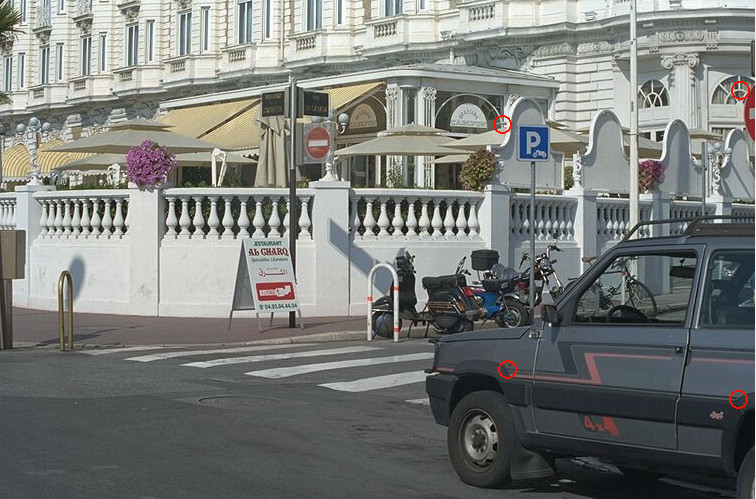
\includegraphics[width = 0.5\textwidth]{I1_2.png} &
% 			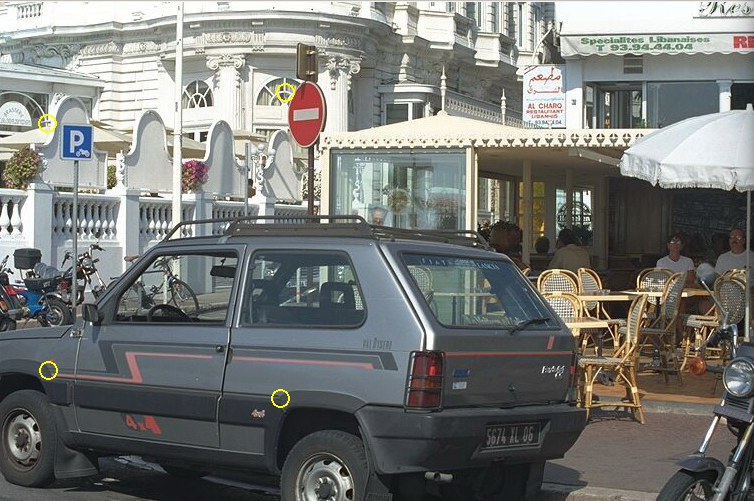
\includegraphics[width = 0.5\textwidth]{I2_2.png}   \\
% 			\multicolumn{2}{c}{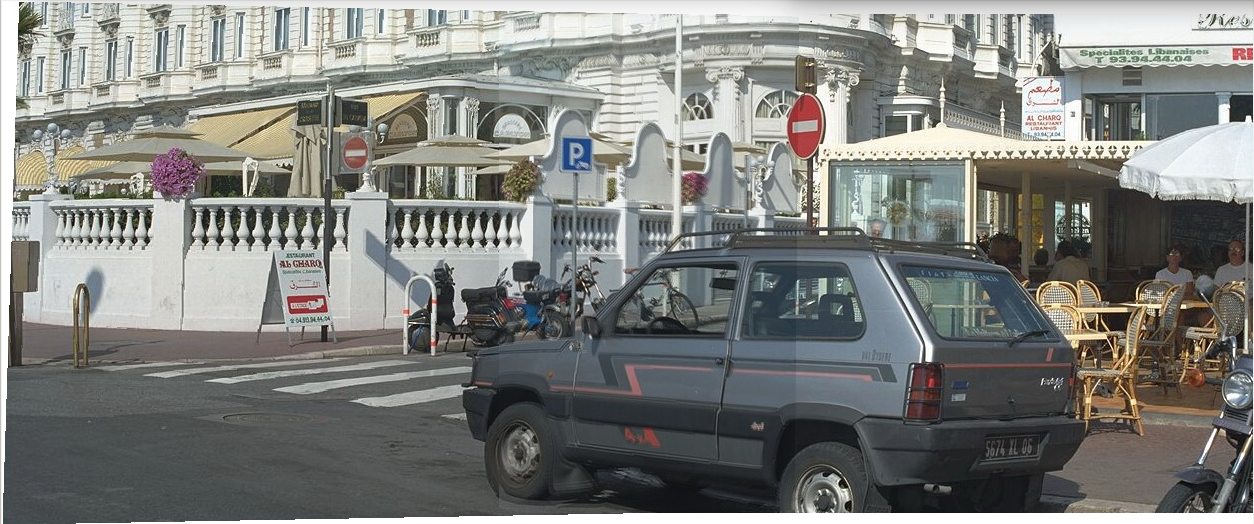
\includegraphics[width = 1.0\textwidth]{Panorama_2.png}}
% 		\end{tabular}
% 	\end{center}
% 	\caption{Top left : first view of the scene. Top right : second view of the scene. Top : circles highlight the correspondances. Bottom : panorama construction with the given correspondances. Size : 1254 x 524}
% 	\label{mini_corr}
% \end{figure}
%
% \subsection{With more than 4 correspondanecs}
%
% In figure \ref{many_corr}, 10 correspondences allow to find an almost perfect homography between the two views. The overlapping area is nearly not blurred, and the panorama format is almost rectangular, which corresponds to a rotation of the view between the optical center.
%
% \subsection{With 4 correspondances}
% \begin{figure}[H]
% 	\begin{center}
% 		\begin{tabular}{p{0.5\textwidth}  p{0.5\textwidth}}
% 			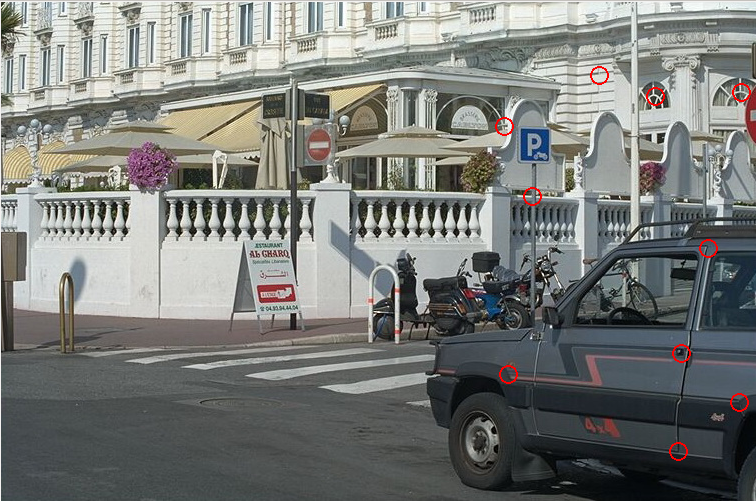
\includegraphics[width = 0.5\textwidth]{I1_3.png} &
% 			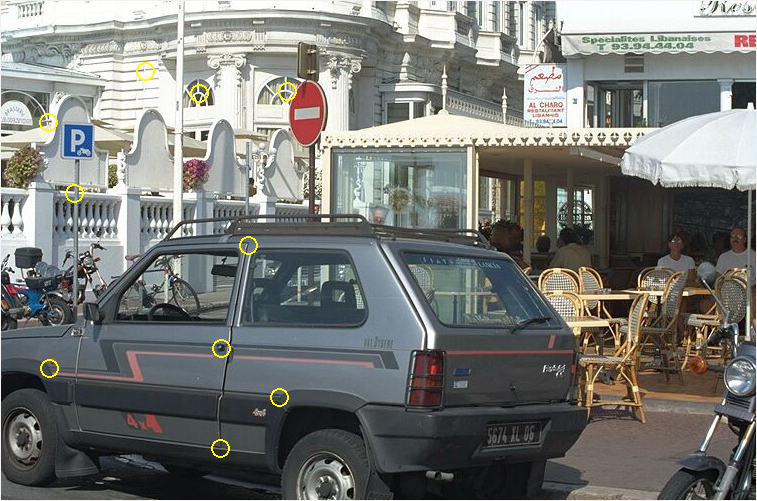
\includegraphics[width = 0.5\textwidth]{I2_3.png}   \\
% 			\multicolumn{2}{c}{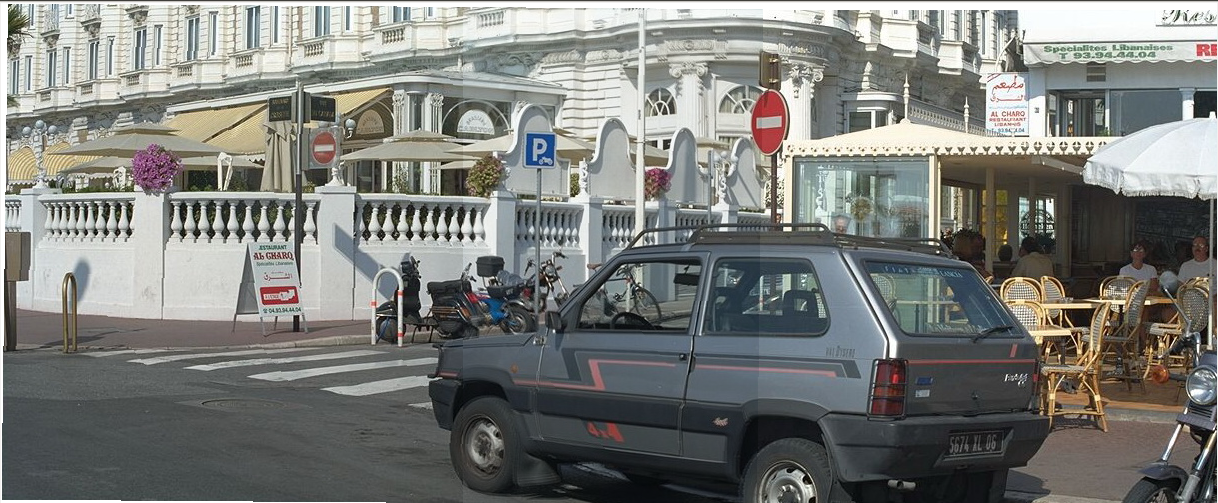
\includegraphics[width = 1.0\textwidth]{Panorama_3.png}}
% 		\end{tabular}
% 	\end{center}
% 	\caption{Top left : first view of the scene. Top right : second view of the scene. Top : circles highlight the correspondances. Bottom : panorama construction with the given correspondances. Size : 1218 x 503}
% 	\label{many_corr}
% \end{figure}

\end{document}
